% Created by tikzDevice version 0.12.3.1 on 2021-12-15 13:58:11
% !TEX encoding = UTF-8 Unicode
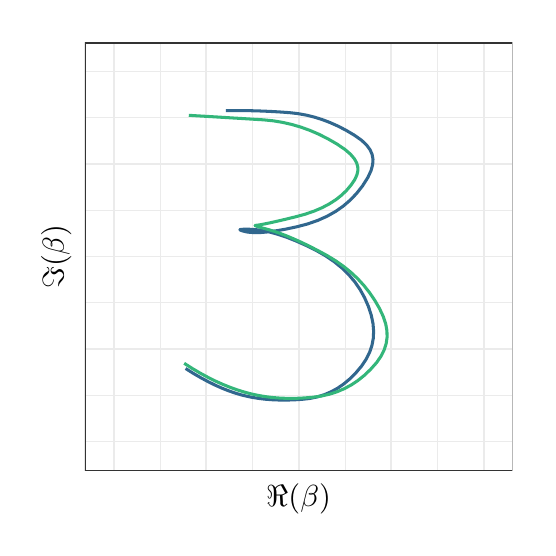
\begin{tikzpicture}[x=1pt,y=1pt]
\definecolor{fillColor}{RGB}{255,255,255}
\path[use as bounding box,fill=fillColor,fill opacity=0.00] (0,0) rectangle (180.67,180.67);
\begin{scope}
\path[clip] (  0.00,  0.00) rectangle (180.67,180.67);
\definecolor{drawColor}{RGB}{255,255,255}
\definecolor{fillColor}{RGB}{255,255,255}

\path[draw=drawColor,line width= 0.6pt,line join=round,line cap=round,fill=fillColor] (  0.00,  0.00) rectangle (180.67,180.68);
\end{scope}
\begin{scope}
\path[clip] ( 20.71, 20.71) rectangle (175.17,175.17);
\definecolor{fillColor}{RGB}{255,255,255}

\path[fill=fillColor] ( 20.71, 20.71) rectangle (175.17,175.17);
\definecolor{drawColor}{gray}{0.92}

\path[draw=drawColor,line width= 0.3pt,line join=round] ( 20.71, 47.80) --
	(175.17, 47.80);

\path[draw=drawColor,line width= 0.3pt,line join=round] ( 20.71, 81.23) --
	(175.17, 81.23);

\path[draw=drawColor,line width= 0.3pt,line join=round] ( 20.71,114.66) --
	(175.17,114.66);

\path[draw=drawColor,line width= 0.3pt,line join=round] ( 20.71,148.09) --
	(175.17,148.09);

\path[draw=drawColor,line width= 0.3pt,line join=round] ( 47.80, 20.71) --
	( 47.80,175.17);

\path[draw=drawColor,line width= 0.3pt,line join=round] ( 81.23, 20.71) --
	( 81.23,175.17);

\path[draw=drawColor,line width= 0.3pt,line join=round] (114.66, 20.71) --
	(114.66,175.17);

\path[draw=drawColor,line width= 0.3pt,line join=round] (148.09, 20.71) --
	(148.09,175.17);

\path[draw=drawColor,line width= 0.6pt,line join=round] ( 20.71, 31.08) --
	(175.17, 31.08);

\path[draw=drawColor,line width= 0.6pt,line join=round] ( 20.71, 64.51) --
	(175.17, 64.51);

\path[draw=drawColor,line width= 0.6pt,line join=round] ( 20.71, 97.94) --
	(175.17, 97.94);

\path[draw=drawColor,line width= 0.6pt,line join=round] ( 20.71,131.38) --
	(175.17,131.38);

\path[draw=drawColor,line width= 0.6pt,line join=round] ( 20.71,164.81) --
	(175.17,164.81);

\path[draw=drawColor,line width= 0.6pt,line join=round] ( 31.08, 20.71) --
	( 31.08,175.17);

\path[draw=drawColor,line width= 0.6pt,line join=round] ( 64.51, 20.71) --
	( 64.51,175.17);

\path[draw=drawColor,line width= 0.6pt,line join=round] ( 97.94, 20.71) --
	( 97.94,175.17);

\path[draw=drawColor,line width= 0.6pt,line join=round] (131.38, 20.71) --
	(131.38,175.17);

\path[draw=drawColor,line width= 0.6pt,line join=round] (164.81, 20.71) --
	(164.81,175.17);
\definecolor{drawColor}{RGB}{49,103,142}

\path[draw=drawColor,line width= 1.1pt,line join=round] ( 57.06, 57.51) --
	( 59.89, 55.73) --
	( 62.61, 54.15) --
	( 65.24, 52.74) --
	( 67.77, 51.49) --
	( 70.20, 50.41) --
	( 72.56, 49.47) --
	( 74.83, 48.68) --
	( 77.02, 48.02) --
	( 79.15, 47.49) --
	( 81.31, 47.05) --
	( 83.55, 46.69) --
	( 85.88, 46.41) --
	( 88.31, 46.22) --
	( 90.84, 46.12) --
	( 93.48, 46.10) --
	( 96.23, 46.18) --
	( 99.10, 46.36) --
	(101.98, 46.69) --
	(104.68, 47.26) --
	(107.24, 48.07) --
	(109.67, 49.11) --
	(112.01, 50.40) --
	(114.27, 51.96) --
	(116.47, 53.81) --
	(118.62, 55.98) --
	(120.74, 58.50) --
	(122.37, 60.97) --
	(123.58, 63.42) --
	(124.41, 65.87) --
	(124.88, 68.38) --
	(125.01, 71.00) --
	(124.78, 73.77) --
	(124.16, 76.74) --
	(123.11, 79.97) --
	(121.73, 83.12) --
	(120.11, 86.05) --
	(118.23, 88.79) --
	(116.07, 91.35) --
	(113.62, 93.77) --
	(110.83, 96.05) --
	(107.68, 98.21) --
	(104.12,100.25) --
	(100.36,102.09) --
	( 96.88,103.63) --
	( 93.67,104.90) --
	( 90.70,105.91) --
	( 87.97,106.68) --
	( 85.45,107.25) --
	( 83.14,107.62) --
	( 81.00,107.81) --
	( 79.03,107.84) --
	( 77.77,107.82) --
	( 77.07,107.77) --
	( 76.77,107.71) --
	( 76.69,107.67) --
	( 76.69,107.64) --
	( 76.81,107.56) --
	( 77.19,107.40) --
	( 78.01,107.13) --
	( 79.15,106.86) --
	( 80.57,106.68) --
	( 82.30,106.61) --
	( 84.38,106.66) --
	( 86.85,106.87) --
	( 89.76,107.26) --
	( 93.14,107.85) --
	( 97.03,108.67) --
	(101.15,109.74) --
	(104.87,111.04) --
	(108.23,112.55) --
	(111.28,114.27) --
	(114.05,116.21) --
	(116.57,118.38) --
	(118.87,120.79) --
	(120.98,123.47) --
	(122.89,126.47) --
	(124.07,129.01) --
	(124.66,131.19) --
	(124.78,133.09) --
	(124.47,134.84) --
	(123.74,136.52) --
	(122.51,138.21) --
	(120.66,139.98) --
	(118.01,141.84) --
	(115.08,143.57) --
	(112.18,145.08) --
	(109.29,146.37) --
	(106.42,147.46) --
	(103.54,148.36) --
	(100.66,149.07) --
	( 97.75,149.60) --
	( 94.81,149.94) --
	( 91.85,150.16) --
	( 88.91,150.34) --
	( 85.98,150.48) --
	( 83.07,150.60) --
	( 80.19,150.67) --
	( 77.31,150.72) --
	( 74.46,150.73) --
	( 71.62,150.71) --
	( 71.62,150.71);
\definecolor{drawColor}{RGB}{51,182,122}

\path[draw=drawColor,line width= 1.1pt,line join=round] ( 56.56, 59.39) --
	( 59.44, 57.55) --
	( 62.26, 55.88) --
	( 65.03, 54.38) --
	( 67.74, 53.02) --
	( 70.40, 51.82) --
	( 73.02, 50.76) --
	( 75.60, 49.83) --
	( 78.14, 49.03) --
	( 80.65, 48.36) --
	( 83.19, 47.81) --
	( 85.80, 47.36) --
	( 88.47, 47.03) --
	( 91.21, 46.81) --
	( 94.04, 46.71) --
	( 96.95, 46.73) --
	( 99.96, 46.87) --
	(103.07, 47.13) --
	(106.17, 47.57) --
	(109.09, 48.23) --
	(111.83, 49.12) --
	(114.44, 50.23) --
	(116.93, 51.58) --
	(119.33, 53.18) --
	(121.64, 55.03) --
	(123.89, 57.18) --
	(126.08, 59.64) --
	(127.70, 61.99) --
	(128.83, 64.27) --
	(129.54, 66.51) --
	(129.87, 68.77) --
	(129.82, 71.12) --
	(129.38, 73.61) --
	(128.49, 76.31) --
	(127.09, 79.27) --
	(125.39, 82.20) --
	(123.52, 84.95) --
	(121.48, 87.53) --
	(119.25, 89.96) --
	(116.82, 92.24) --
	(114.17, 94.40) --
	(111.29, 96.43) --
	(108.16, 98.34) --
	(104.91,100.10) --
	(101.85,101.68) --
	( 98.97,103.07) --
	( 96.27,104.29) --
	( 93.74,105.36) --
	( 91.36,106.27) --
	( 89.14,107.05) --
	( 87.06,107.69) --
	( 85.12,108.21) --
	( 83.78,108.59) --
	( 82.92,108.87) --
	( 82.44,109.04) --
	( 82.23,109.14) --
	( 82.17,109.18) --
	( 82.17,109.20) --
	( 82.24,109.22) --
	( 82.48,109.24) --
	( 82.93,109.29) --
	( 83.64,109.39) --
	( 84.67,109.57) --
	( 86.06,109.84) --
	( 87.88,110.22) --
	( 90.18,110.74) --
	( 93.03,111.40) --
	( 96.47,112.24) --
	(100.20,113.24) --
	(103.52,114.39) --
	(106.46,115.65) --
	(109.06,117.03) --
	(111.37,118.51) --
	(113.40,120.12) --
	(115.20,121.84) --
	(116.78,123.70) --
	(118.16,125.71) --
	(118.96,127.44) --
	(119.31,128.99) --
	(119.27,130.42) --
	(118.87,131.83) --
	(118.03,133.32) --
	(116.66,134.93) --
	(114.60,136.71) --
	(111.68,138.67) --
	(108.45,140.53) --
	(105.22,142.16) --
	(101.99,143.55) --
	( 98.73,144.73) --
	( 95.44,145.69) --
	( 92.11,146.45) --
	( 88.73,147.01) --
	( 85.28,147.36) --
	( 81.78,147.57) --
	( 78.32,147.79) --
	( 74.90,147.99) --
	( 71.50,148.20) --
	( 68.13,148.41) --
	( 64.80,148.61) --
	( 61.50,148.80) --
	( 58.23,149.00) --
	( 58.23,149.00);
\definecolor{drawColor}{gray}{0.20}

\path[draw=drawColor,line width= 0.6pt,line join=round,line cap=round] ( 20.71, 20.71) rectangle (175.17,175.17);
\end{scope}
\begin{scope}
\path[clip] (  0.00,  0.00) rectangle (180.67,180.67);
\definecolor{drawColor}{RGB}{0,0,0}

\node[text=drawColor,anchor=base,inner sep=0pt, outer sep=0pt, scale=  1.10] at ( 97.94,  7.64) {$\Re(\beta)$};
\end{scope}
\begin{scope}
\path[clip] (  0.00,  0.00) rectangle (180.67,180.67);
\definecolor{drawColor}{RGB}{0,0,0}

\node[text=drawColor,rotate= 90.00,anchor=base,inner sep=0pt, outer sep=0pt, scale=  1.10] at ( 13.08, 97.94) {$\Im(\beta)$};
\end{scope}
\end{tikzpicture}
